\documentclass[10pt]{article}
 
\usepackage[margin=1.5cm]{geometry} 
\usepackage{amsmath,amsthm,amssymb}
%\usepackage{hyperref}
\usepackage{graphicx}
\usepackage{tabularx}
\usepackage{multirow}
\usepackage{float}
\usepackage{subfig}

\setlength{\parindent}{0pt}
\graphicspath{{./images/}}

\begin{document}

% --------------------------------------------------------------
%                         Start here
% --------------------------------------------------------------
  
\title{Big Data Computing - $4^{th}$ Homework Report}
\author{Boem Davide, ID: 1176946, \texttt{davide.boem@studenti.unipd.it} \and Boscaro Nicola, ID: 1181356, \texttt{nicola.boscaro.1@studenti.unipd.it} \and Faccin Dario, ID: 1177736, \texttt{dario.faccin@studenti.unipd.it}\footnote{Contact email}}
\date{}
 
\maketitle

In this report we described the results obtained by running our code, on \textit{Cloud Veneto}, for the $4^{th}$ homework.

\section{Results}

In Table \ref{tab:results1} you can see what we have obtained running our code on \textit{Cloud Veneto}\footnote{We decided to round the average distances to 4 decimal places.}.

\begin{table}[H]
  \centering
  \begin{tabularx}{\textwidth}{c || p{1.5cm} | p{1.5cm} | c | c | p{1.7cm} | p{2.2cm} | p{1.5cm} | p{2cm} }
    & \textbf{Cores used by application} & \textbf{Cores used for each executor} & \textbf{numBlocks} & \textbf{k} & \textbf{Coreset construction (ms)} & \textbf{Computation final solution (ms)} & \textbf{Average distance} & \textbf{Dataset (Approximate size)}\\
\hline\hline
\textbf{1} & \centering 20 & \centering 4 & 12 & 10 & \centering 26519 & \centering 24 & \centering 10,5483 & \multirow{10}{*}{\centering\texttt{all}}\\
\textbf{2} & \centering 20 & \centering 4 & 12 & 20 & \centering 25519 & \centering 40 & \centering 9,9642 & \\
\textbf{3} & \centering 20 & \centering 4 & 12 & 30 & \centering 23942 & \centering 70 & \centering 9,7861 & \\
\textbf{4} & \centering 20 & \centering 4 & 12 & 40 & \centering 25159 & \centering 155 & \centering 9,6639 & \\
\textbf{5} & \centering 20 & \centering 4 & 12 & 50 & \centering 23727 & \centering 297 & \centering 9,5462 & \\
\textbf{6} & \centering 20 & \centering 4 & 12 & 60 & \centering 30821 & \centering 449 & \centering 9,4961 & \\
\textbf{7} & \centering 20 & \centering 4 & 12 & 70 & \centering 25678 & \centering 726 & \centering 9,3317 & \\
\textbf{8} & \centering 20 & \centering 4 & 12 & 80 & \centering 27404 & \centering 1060 & \centering 9,3204 & \\
\textbf{9} & \centering 20 & \centering 4 & 12 & 90 & \centering 37561 & \centering 1527 & \centering 9,2578 & \\
\textbf{10} & \centering 20 & \centering 4 & 12 & 100 & \centering 32148 & \centering 2122 & \centering 9,1879 & \\
%\textbf{11} & \centering 20 & \centering 4 & 12 & 110 & \centering 68265 & \centering 2818 & \centering 9,1743 & \\
%\textbf{12} & \centering 20 & \centering 4 & 12 & 120 & \centering 73367 & \centering 3578 & \centering 9,1061 & \\
%\textbf{13} & \centering 20 & \centering 4 & 12 & 130 & \centering 59042 & \centering 4454 & \centering 9,0946 & \\
%\textbf{14} & \centering 20 & \centering 4 & 12 & 140 & \centering 62462 & \centering 5745 & \centering 9,0689 & \\
%\textbf{15} & \centering 20 & \centering 4 & 12 & 150 & \centering 48574 & \centering 8027 & \centering 9,0431 & \\
%\textbf{16} & \centering 20 & \centering 4 & 12 & 160 & \centering 36865 & \centering 12089 & \centering 9,0115 & \\
%\textbf{17} & \centering 20 & \centering 4 & 12 & 170 & \centering 56385 & \centering 11927 & \centering 8,9946 & \\
%\textbf{18} & \centering 20 & \centering 4 & 12 & 180 & \centering 52730 & \centering 12659 & \centering 8,9458 & \\
%\textbf{19} & \centering 20 & \centering 4 & 12 & 190 & \centering 69069 & \centering 14400 & \centering 8,9466 & \\ 
%\textbf{20} & \centering 20 & \centering 4 & 12 & 200 & \centering 82165 & \centering 16747 & \centering 8,9113 & \\
  \end{tabularx}
  \caption{Results obtained on \textit{Cloud Veneto}, using dataset \texttt{vectors-50-all.txt.bz2} and changing $k$.} \label{tab:results1}
\end{table}

\begin{table}[H]
  \centering
  \begin{tabularx}{\textwidth}{c || p{1.5cm} | p{1.5cm} | c | c | p{1.7cm} | p{2.2cm} | p{1.5cm} | p{2cm} }
    & \textbf{Cores used by application} & \textbf{Cores used for each executor} & \textbf{numBlocks} & \textbf{k} & \textbf{Coreset construction (ms)} & \textbf{Computation final solution (ms)} & \textbf{Average distance} & \textbf{Dataset (Approximate size)}\\
\hline\hline
\textbf{1} & \centering 20 & \centering 4 & 12 & 10 & \centering 12636 & \centering 43 & \centering 10,2092 & \multirow{10}{*}{\centering\texttt{2000000}}\\
\textbf{2} & \centering 20 & \centering 4 & 12 & 20 & \centering 9732 & \centering 103 & \centering 9,5775 & \\
\textbf{3} & \centering 20 & \centering 4 & 12 & 30 & \centering 14897 & \centering 109 & \centering 9,2798 & \\
\textbf{4} & \centering 20 & \centering 4 & 12 & 40 & \centering 12534 & \centering 172 & \centering 9,0856 & \\
\textbf{5} & \centering 20 & \centering 4 & 12 & 50 & \centering 14074 & \centering 484 & \centering 8,9951 & \\
\textbf{6} & \centering 20 & \centering 4 & 12 & 60 & \centering 18627 & \centering 455 & \centering 8,9671 & \\
\textbf{7} & \centering 20 & \centering 4 & 12 & 70 & \centering 23357 & \centering 876 & \centering 8,9588 & \\
\textbf{8} & \centering 20 & \centering 4 & 12 & 80 & \centering 24393 & \centering 1141 & \centering 8,9301 & \\
\textbf{9} & \centering 20 & \centering 4 & 12 & 90 & \centering 30550 & \centering 1790 & \centering 8,8520 & \\
\textbf{10} & \centering 20 & \centering 4 & 12 & 100 & \centering 22076 & \centering 2093 & \centering 8,8300 & \\
  \end{tabularx}
  \caption{Results obtained on \textit{Cloud Veneto}, using dataset \texttt{vectors-50-2000000.txt.bz2} and changing $k$.} \label{tab:results2}
\end{table}

\iffalse
\begin{table}[H]
  \centering
  \begin{tabularx}{\textwidth}{c || p{1.5cm} | p{1.5cm} | c | c | p{1.7cm} | p{2.2cm} | p{1.5cm} | p{2cm} }
    & \textbf{Cores used by application} & \textbf{Cores used for each executor} & \textbf{numBlocks} & \textbf{k} & \textbf{Coreset construction (ms)} & \textbf{Computation final solution (ms)} & \textbf{Average distance} & \textbf{Dataset (Approximate size)}\\
\hline\hline
\textbf{1} & \centering 20 & \centering 4 & 10 & 20 & \centering 11781 & \centering 49 & \centering 10,1422 & \multirow{20}{*}{\centering\texttt{all}}\\
\textbf{2} & \centering 20 & \centering 4 & 20 & 20 & \centering 33848 & \centering 56 & \centering 10,0583 & \\
\textbf{3} & \centering 20 & \centering 4 & 30 & 20 & \centering 32841 & \centering 130 & \centering 9,9066 & \\
\textbf{4} & \centering 20 & \centering 4 & 40 & 20 & \centering 6576 & \centering 198 & \centering 9,9467 & \\
\textbf{5} & \centering 20 & \centering 4 & 50 & 20 & \centering 29907 & \centering 335 & \centering 9,7920 & \\
\textbf{6} & \centering 20 & \centering 4 & 60 & 20 & \centering 7354 & \centering 510 & \centering 9,7920 & \\
\textbf{7} & \centering 20 & \centering 4 & 70 & 20 & \centering 8124 & \centering 642 & \centering 9,9569 & \\
\textbf{8} & \centering 20 & \centering 4 & 80 & 20 & \centering 8689 & \centering 814 & \centering 9,8959 & \\
\textbf{9} & \centering 20 & \centering 4 & 90 & 20 & \centering 6466 & \centering 1082 & \centering 9,9125 & \\
\textbf{10} & \centering 20 & \centering 4 & 100 & 20 & \centering 6641 & \centering 1235 & \centering 9,9389 & \\
\textbf{11} & \centering 20 & \centering 4 & 110 & 20 & \centering 7016 & \centering 1631 & \centering 9,7920 & \\
\textbf{12} & \centering 20 & \centering 4 & 120 & 20 & \centering 6636 & \centering 2041 & \centering 9,7920 & \\
\textbf{13} & \centering 20 & \centering 4 & 130 & 20 & \centering 7867 & \centering 3309 & \centering 9,9125 & \\
\textbf{14} & \centering 20 & \centering 4 & 140 & 20 & \centering 7058 & \centering 2955 & \centering 9,7920 & \\
\textbf{15} & \centering 20 & \centering 4 & 150 & 20 & \centering 6314 & \centering 2992 & \centering 9,7920 & \\
\textbf{16} & \centering 20 & \centering 4 & 160 & 20 & \centering 9296 & \centering 4145 & \centering 9,7920 & \\
\textbf{17} & \centering 20 & \centering 4 & 170 & 20 & \centering 8206 & \centering 4552 & \centering 9,7920 & \\
\textbf{18} & \centering 20 & \centering 4 & 180 & 20 & \centering 6821 & \centering 6880 & \centering 9,7920 & \\
\textbf{19} & \centering 20 & \centering 4 & 190 & 20 & \centering 8734 & \centering 9796 & \centering 9,7920 & \\ 
\textbf{20} & \centering 20 & \centering 4 & 200 & 20 & \centering 8407 & \centering 9755 & \centering 9,7920 & \\
  \end{tabularx}
  \caption{Results obtained on \textit{Cloud Veneto}, using dataset \texttt{vectors-50-all.txt.bz2} and changing $numBlocks$.} \label{tab:results3}
\end{table}

\begin{table}[H]
  \centering
  \begin{tabularx}{\textwidth}{c || p{1.5cm} | p{1.5cm} | c | c | p{1.7cm} | p{2.2cm} | p{1.5cm} | p{2cm} }
    & \textbf{Cores used by application} & \textbf{Cores used for each executor} & \textbf{numBlocks} & \textbf{k} & \textbf{Coreset construction (ms)} & \textbf{Computation final solution (ms)} & \textbf{Average distance} & \textbf{Dataset (Approximate size)}\\
\hline\hline
\textbf{1} & \centering 20 & \centering 4 & 10 & 20 & \centering 5160 & \centering 66 & \centering 9,5939 & \multirow{10}{*}{\centering\texttt{2000000}}\\
\textbf{2} & \centering 20 & \centering 4 & 20 & 20 & \centering 3659 & \centering 118 & \centering 9,6041 & \\
\textbf{3} & \centering 20 & \centering 4 & 30 & 20 & \centering 3598 & \centering 224 & \centering 9,5847 & \\
\textbf{4} & \centering 20 & \centering 4 & 40 & 20 & \centering 3077 & \centering 273 & \centering 9,4245 & \\
\textbf{5} & \centering 20 & \centering 4 & 50 & 20 & \centering 3033 & \centering 448 & \centering 9,5375 & \\
\textbf{6} & \centering 20 & \centering 4 & 60 & 20 & \centering 3634 & \centering 678 & \centering 9,7332 & \\
\textbf{7} & \centering 20 & \centering 4 & 70 & 20 & \centering 3129 & \centering 909 & \centering 9,4245 & \\
\textbf{8} & \centering 20 & \centering 4 & 80 & 20 & \centering 3238 & \centering 913 & \centering 9,4245 & \\
\textbf{9} & \centering 20 & \centering 4 & 90 & 20 & \centering 3097 & \centering 1709 & \centering 9,4245 & \\
\textbf{10} & \centering 20 & \centering 4 & 100 & 20 & \centering 4176 & \centering 1596 & \centering 9,4245 & \\
  \end{tabularx}
  \caption{Results obtained on \textit{Cloud Veneto}, using dataset \texttt{vectors-50-2000000.txt.bz2} and changing $numBlocks$.} \label{tab:results4}
\end{table}

\begin{table}[H]
  \centering
  \begin{tabularx}{\textwidth}{c || p{1.5cm} | p{1.5cm} | c | c | p{1.7cm} | p{2.2cm} | p{1.5cm} | p{2cm} }
    & \textbf{Cores used by application} & \textbf{Cores used for each executor} & \textbf{numBlocks} & \textbf{k} & \textbf{Coreset construction (ms)} & \textbf{Computation final solution (ms)} & \textbf{Average distance} & \textbf{Dataset (Approximate size)}\\
\hline\hline
\textbf{1} & \centering 30 & \centering 4 & 12 & 10 & \centering 12951 & \centering 34 & \centering 10,5483 & \multirow{10}{*}{\centering\texttt{all}}\\
\textbf{2} & \centering 30 & \centering 4 & 12 & 20 & \centering 16580 & \centering 42 & \centering 10,1264 & \\
\textbf{3} & \centering 30 & \centering 4 & 12 & 30 & \centering 18378 & \centering 129 & \centering 9,8571 & \\
\textbf{4} & \centering 30 & \centering 4 & 12 & 40 & \centering 25320 & \centering 181 & \centering 9,6896 & \\
\textbf{5} & \centering 30 & \centering 4 & 12 & 50 & \centering 24738 & \centering 350 & \centering 9,5100 & \\
\textbf{6} & \centering 30 & \centering 4 & 12 & 60 & \centering 37329 & \centering 465 & \centering 9,4490 & \\
\textbf{7} & \centering 30 & \centering 4 & 12 & 70 & \centering 40478 & \centering 842 & \centering 9,3427 & \\
\textbf{8} & \centering 30 & \centering 4 & 12 & 80 & \centering 37355 & \centering 1170 & \centering 9,3359 & \\
\textbf{9} & \centering 30 & \centering 4 & 12 & 90 & \centering 33338 & \centering 1926 & \centering 9,1828 & \\
\textbf{10} & \centering 30 & \centering 4 & 12 & 100 & \centering 36045 & \centering 2570 & \centering 9,1724 & \\
  \end{tabularx}
  \caption{Results obtained on \textit{Cloud Veneto}, using dataset \texttt{vectors-50-all.txt.bz2} and changing $X$.} \label{tab:results5}
\end{table}

\begin{table}[H]
  \centering
  \begin{tabularx}{\textwidth}{c || p{1.5cm} | p{1.5cm} | c | c | p{1.7cm} | p{2.2cm} | p{1.5cm} | p{2cm} }
    & \textbf{Cores used by application} & \textbf{Cores used for each executor} & \textbf{numBlocks} & \textbf{k} & \textbf{Coreset construction (ms)} & \textbf{Computation final solution (ms)} & \textbf{Average distance} & \textbf{Dataset (Approximate size)}\\
\hline\hline
\textbf{1} & \centering 20 & \centering 8 & 12 & 10 & \centering 47584 & \centering 54 & \centering 10,6549 & \multirow{10}{*}{\centering\texttt{all}}\\
\textbf{2} & \centering 20 & \centering 8 & 12 & 20 & \centering 47944 & \centering 48 & \centering 10,1581 & \\
\textbf{3} & \centering 20 & \centering 8 & 12 & 30 & \centering 60405 & \centering 101 & \centering 9,8100 & \\
\textbf{4} & \centering 20 & \centering 8 & 12 & 40 & \centering 51350 & \centering 146 & \centering 9,7196 & \\
\textbf{5} & \centering 20 & \centering 8 & 12 & 50 & \centering 50555 & \centering 266 & \centering 9,5379 & \\
\textbf{6} & \centering 20 & \centering 8 & 12 & 60 & \centering 61062 & \centering 735 & \centering 9,4922 & \\
\textbf{7} & \centering 20 & \centering 8 & 12 & 70 & \centering 52542 & \centering 932 & \centering 9,3342 & \\
\textbf{8} & \centering 20 & \centering 8 & 12 & 80 & \centering 59816 & \centering 1614 & \centering 9,3254 & \\
\textbf{9} & \centering 20 & \centering 8 & 12 & 90 & \centering 62616 & \centering 2101 & \centering 9,2225 & \\
\textbf{10} & \centering 20 & \centering 8 & 12 & 100 & \centering 59043 & \centering 2146 & \centering 9,2218 & \\
  \end{tabularx}
  \caption{Results obtained on \textit{Cloud Veneto}, using dataset \texttt{vectors-50-all.txt.bz2} and changing $Y$.} \label{tab:results6}
\end{table}
\fi


\section{Plots}

\begin{figure}[H]
	\centering
	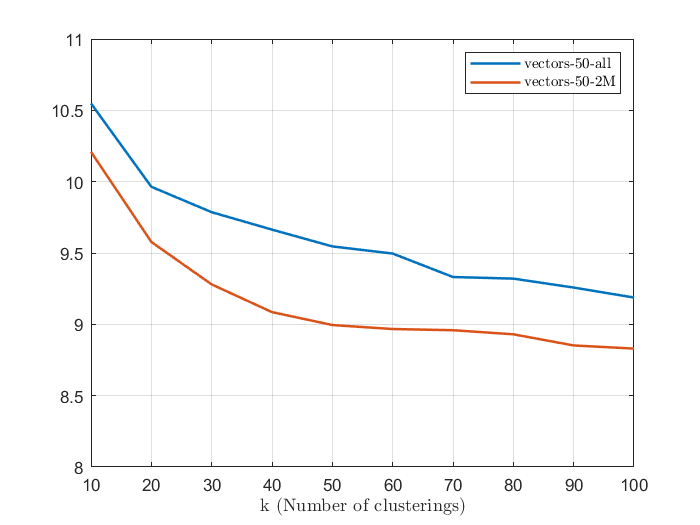
\includegraphics[width=8cm]{maxdivdst}
	\caption{Max diversity distance computed for two datasets.}
\end{figure}

\begin{figure}[H]
	\centering
	\subfloat[Times for 5 millions vectors.]{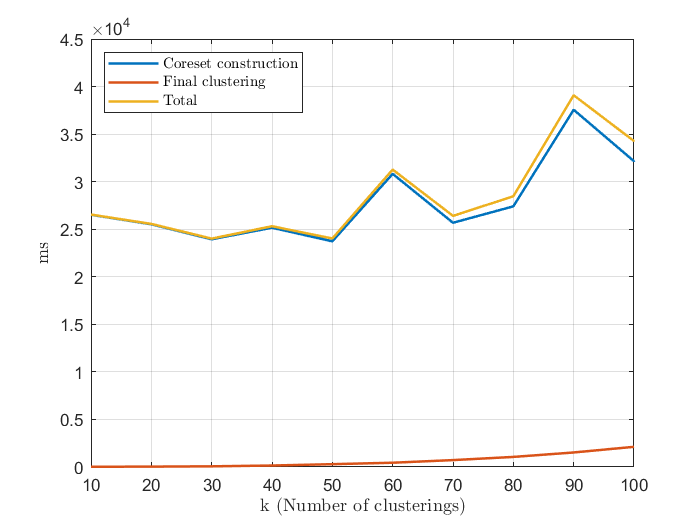
\includegraphics[width=8cm]{times_all_vects}}
	\subfloat[Times for 2 millions vectors.]{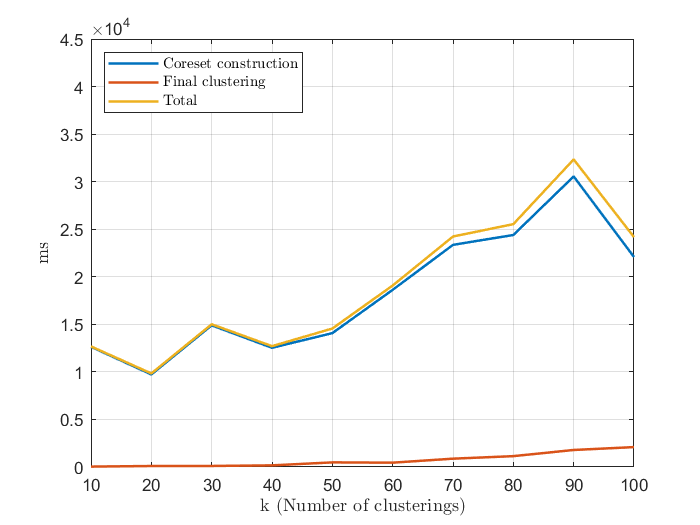
\includegraphics[width=8cm]{times_2M_vects}}
	\caption{Execution times for two datasets.}
\end{figure}

\section{Conclusions}

Looking at the results (see Table \ref{tab:results1}), we can see that, while the measured time for the \textit{Construction of the coreset} remains almost inside a time interval, the time spent by the program for the \textit{Computation of the final solution} rises proportionally with the values of $k$ and of $numBlocks$.

On the contrary, the \textit{Average distance} starts with bigger values and converges after a while to lower values.

In the case of the total number of cores used by the application ($X$) we observed that there was a little improvement in the measured time of the \textit{Construction of the coreset}, meanwhile, modifying the number of cores used for each executor ($Y$) we didn't see any enhancement.
\end{document}